\begin{figure}[t]
\centering
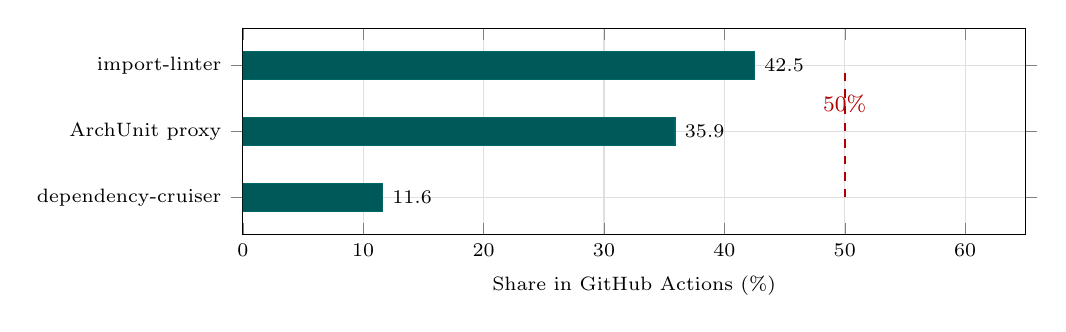
\begin{tikzpicture}
\begin{axis}[
  xbar,
  width=0.95\columnwidth,
  height=4.2cm,
  xmin=0, xmax=65,
  xlabel={Share in GitHub Actions (\%)},
  symbolic y coords={dependency-cruiser,ArchUnit proxy,import-linter},
  ytick=data,
  nodes near coords,
  nodes near coords align={horizontal},
  every node near coord/.append style={font=\scriptsize},
  bar width=10pt,
  enlarge y limits=0.28,
  grid=major,
  major grid style={gray!25},
  tick label style={font=\scriptsize},
  label style={font=\scriptsize},
]
\addplot[fill=teal!70!black, draw=teal!80!black] coordinates {
  (42.5,import-linter)
  (35.9,{ArchUnit proxy})
  (11.6,dependency-cruiser)
};
\draw[dashed, red!70!black, thick]
  (axis cs:50,dependency-cruiser) -- (axis cs:50,import-linter)
  node[above, font=\footnotesize, red!70!black, midway, yshift=3pt] {$50\%$};
\end{axis}
\end{tikzpicture}
\caption{GitHub Actions integration rates by tool. The ArchUnit bar represents a Maven or Gradle build-or-test proxy rather than direct evidence of ArchUnit rule execution. The dashed line indicates the hypothesized threshold of 50\%.}
\label{fig:ci_share}
\end{figure}